%%%%%%%%%%%%%%%%%%%%%%%%%%%%%%%%%%%%%%%%%%%%%%%%%%%%%%%%%%%%%%%%%%%%%%%%%
%  This file controls your whole document. It has three functions:
%     1. Include and configure any packages used in the document
%     2. Define page numbering, structure and bibliography
%     3. Import/Include all other files
%
%  More information is provided in the README.md
%
%  Written by M. Imran 2001/06/18
%  No Copyright for this file. Save your time and enjoy it 
%  Updated by Ian Craig 2014/10/20 for UNSW Mech Eng Thesis guidelines 
%%%%%%%%%%%%%%%%%%%%%%%%%%%%%%%%%%%%%%%%%%%%%%%%%%%%%%%%%%%%%%%%%%%%%%%%%

\documentclass[thesis]{unswthesis}

% % % USE PACKAGES % % % % % % % % % % % % % % % % % % % % % % % % % % % % % %
\usepackage{usnomencl} % For making a glossary of nomenclature.
\usepackage{graphics}
\usepackage{graphicx}
\usepackage{caption}
\usepackage{subcaption} % Replaces subfig and subfigure.
\usepackage{amssymb}
\usepackage{amsmath}
\usepackage{url}
\urlstyle{rm}
\usepackage{booktabs} % From http://goo.gl/2ezu9p to make tables look nicer.
\usepackage{mathtext}
\usepackage{multirow}
\usepackage{fmtcount}
\usepackage{ctable}
\usepackage{array}
\usepackage{epstopdf}
\usepackage[draft]{listofsymbols} % Added 120605 to add list of symbols
\usepackage{fancyhdr}
\usepackage{epsfig}
\usepackage{cite}
\usepackage{theorem}
\usepackage{color}
\usepackage{hyperref}
\usepackage{latexsym}
\usepackage{epic}
\usepackage{setspace}
\usepackage{mdwlist} % For reducing list vertical spacing. http://goo.gl/nyLux
\usepackage{pdflscape} % Make landscape pages display rotated in PDFs http://goo.gl/wbg4fy
\usepackage{algorithm}
\usepackage{algpseudocode} % To display algorithms nicely. http://goo.gl/6Z93aV
\usepackage{printlen} % To print variables. http://goo.gl/3ZdAPV
%\uselengthunit{in} % See above
%\printlength{\textwidth} % See above
%\the\textwidth   % \textwidth = 426.79134 pt = 149.99823 mm = 5.90666 in. An alternative method of printing variables.
% @300dpi --> 1771 px.
% % For adding Latex Section symbols to the actual headings:
%\usepackage{titlesec}. 
%\titleformat{\section}{\normalfont\Large\bfseries}{\S\thesection}{1em}{}
% % For cyrillic font (naiive i)
%\usepackage[OT2,OT1]{fontenc} 
% % % END PACKAGES % % % % % % % % % % % % % % % % % % % % % % % % % % % % % %

% Setup
%%%%%%%%%%%%%%%%%%%%%%%%%%%%%%%%%%%%%%%%%%%%%%%%%%%%%%%%%%%%%%%%%%%%%%%%%%
%  This is format.tex file needed for the unswthesis.cls file.           %
%  It defines the part of style and formatting for the document which is % 
%  configurable. The remaining style is defined by unswthesis.cls but    %
%  you should not need to worry about this :)                            %
%                                                                        %
%  Written by M. Imran 2001/06/18                                        %
%  No Copyright for this file. Save your time and enjoy it               %
%  Updated by Ian Craig 2014/10/20 for UNSW Mech Eng Thesis guidelines   %
%%%%%%%%%%%%%%%%%%%%%%%%%%%%%%%%%%%%%%%%%%%%%%%%%%%%%%%%%%%%%%%%%%%%%%%%%%
%%%%%  Put packages you want to use here and 'fancyhdr' is required   %%%%
%%%%%%%%%%%%%%%%%%%%%%%%%%%%%%%%%%%%%%%%%%%%%%%%%%%%%%%%%%%%%%%%%%%%%%%%%%


%\hlopts{bwidth=0}
%\hlopts[url]{colormodel=named,color=BlueViolet}
%\hypersetup{linkcolor=cyan,citecolor=cyan,urlcolor=cyan}
%%%%%%%%%%%%%%%%%%%%%%%%%%%%%%%%%%%%%%%%%%%%%%%%%%%%%%%%%%%%%%%%%%%%%%%%%%
%%%%%                      Your fancy heading                       %%%%%%
%%%%% For the final copy you need to remove '\bfseries\today' below %%%%%%
%%%%%%%%%%%%%%%%%%%%%%%%%%%%%%%%%%%%%%%%%%%%%%%%%%%%%%%%%%%%%%%%%%%%%%%%%%
\pagestyle{fancy}
\renewcommand{\chaptermark}[1]{\markright{\chaptername\ \thechapter.\ #1}}
\renewcommand{\sectionmark}[1]{\markright{\thesection.\ #1}{}}
\lhead[\fancyplain{}{}]%
      {\fancyplain{}{\bfseries\rightmark}}
\chead[\fancyplain{}{}]%
      {\fancyplain{}{}}
\rhead[\fancyplain{}{}]%
      {\fancyplain{}{\bfseries\thepage}}
\lfoot[\fancyplain{}{}]%
      {\fancyplain{}{}}
\cfoot[\fancyplain{}{}]%
      {\fancyplain{}{}}
\rfoot[\fancyplain{}{}]%
      {\fancyplain{}{\bfseries\today}}
%%%%%%%%%%%%%%%%%%%%%%%%%%%%%%%%%%%%%%%%%%%%%%%%%%%%%%%%%%%%%%%%%%%%%%%%%%
%%%%%%%%%%%%Here you set the space between the main text%%%%%%%%%%%%%%%%%%
%%%%%%%%%%%%%%%%%%%and the start of the footnote%%%%%%%%%%%%%%%%%%%%%%%%%%
%%%%%%%%%%%%%%%%%%%%%%%%%%%%%%%%%%%%%%%%%%%%%%%%%%%%%%%%%%%%%%%%%%%%%%%%%%
\addtolength{\skip\footins}{5mm}
%%%%%%%%%%%%%%%%%%%%%%%%%%%%%%%%%%%%%%%%%%%%%%%%%%%%%%%%%%%%%%%%%%%%%%%%%%
%%%%%      Define new counter so you can have the equation           %%%%%
%%%%%    number 4.2.1a for example, this a gift from J.F.Blowey      %%%%%
%%%%%%%%%%%%%%%%%%%%%%%%%%%%%%%%%%%%%%%%%%%%%%%%%%%%%%%%%%%%%%%%%%%%%%%%%%
\newcounter{ind}
\def\eqlabon{
\setcounter{ind}{\value{equation}}\addtocounter{ind}{1}
\setcounter{equation}{0}
\renewcommand{\theequation}{\arabic{chapter}%
         .\arabic{section}.\arabic{ind}\alph{equation}}}
\def\eqlaboff{
\renewcommand{\theequation}{\arabic{chapter}%
         .\arabic{section}.\arabic{equation}}
\setcounter{equation}{\value{ind}}}
%%%%%%%%%%%%%%%%%%%%%%%%%%%%%%%%%%%%%%%%%%%%%%%%%%%%%%%%%%%%%%%%%%%%%%%%%%
%%%%%%%%%%%%           New theorem you want to use              %%%%%%%%%%
%%%%%%%%%%%%%%%%%%%%%%%%%%%%%%%%%%%%%%%%%%%%%%%%%%%%%%%%%%%%%%%%%%%%%%%%%%
{\theorembodyfont{\rmfamily}\newtheorem{Pro}{{\textbf Proposition}}[section]}
{\theorembodyfont{\rmfamily}\newtheorem{The}{{\textbf Theorem}}[section]}
{\theorembodyfont{\rmfamily}\newtheorem{Def}[The]{{\textbf Definition}}}
{\theorembodyfont{\rmfamily}\newtheorem{Cor}[The]{{\textbf Corollary}}}
{\theorembodyfont{\rmfamily}\newtheorem{Lem}[The]{{\textbf Lemma}}}
{\theorembodyfont{\rmfamily}\newtheorem{Exp}{{\textbf Example}}[section]}
\def\remark{\textbf{Remark}:}
\def\remarks{\textbf{Remarks}:}
\def\bproof{\textbf{Proof}: }
\def\eproof{\hfill$\Box$}
%%%%%%%%%%%%%%%%%%%%%%%%%%%%%%%%%%%%%%%%%%%%%%%%%%%%%%%%%%%%%%%%%%%%%%%%%%
%%%%%%%    Bold font in math mode, a gift from J.F.Blowey       %%%%%%%%%%
%%%%%%%%%%%%%%%%%%%%%%%%%%%%%%%%%%%%%%%%%%%%%%%%%%%%%%%%%%%%%%%%%%%%%%%%%%
\def\bv#1{\mbox{\boldmath$#1$}}
%%%%%%%%%%%%%%%%%%%%%%%%%%%%%%%%%%%%%%%%%%%%%%%%%%%%%%%%%%%%%%%%%%%%%%%%%%
%%%%%%%        New symbol which is not defined in Latex         %%%%%%%%%%
%%%%%%%                 a gift from J.F.Blowey                  %%%%%%%%%%
%%%%%%%%%%%%%%%%%%%%%%%%%%%%%%%%%%%%%%%%%%%%%%%%%%%%%%%%%%%%%%%%%%%%%%%%%%
% The Mean INTegral
% to be used in displaystyle
\def\mint{\textstyle\mints\displaystyle}
% to be used in textstyle
\def\mints{\int\!\!\!\!\!\!{\rm-}\ }
%
% The Mean SUM
% to be used in displaystyle
\def\msum{\textstyle\msums\displaystyle}
% to be used in textstyle
\def\msums{\sum\!\!\!\!\!\!\!{\rm-}\ }
%%%%%%%%%%%%%%%%%%%%%%%%%%%%%%%%%%%%%%%%%%%%%%%%%%%%%%%%%%%%%%%%%%%%%%%%%%
%%%%%%%%%%            Define your short cut here              %%%%%%%%%%%%
%%%%%%%%%%%%%%%%%%%%%%%%%%%%%%%%%%%%%%%%%%%%%%%%%%%%%%%%%%%%%%%%%%%%%%%%%%
\def\poincare{Poincar\'e }
\def\holder{H\"older }
%%%%%%%%%%%%%%%%%%%%%%%%%%%%%%%%%%%%%%%%%%%%%%%%%%%%%%%%%%%%%%%%%%%%%%%%%%
%%%%%%%%%%            small font captions             				%%%%%%%%%%%%
%%%%%%%%%%%%%%%%%%%%%%%%%%%%%%%%%%%%%%%%%%%%%%%%%%%%%%%%%%%%%%%%%%%%%%%%%%
% Different font in captions
\newcommand{\captionfonts}{\small}

\makeatletter  % Allow the use of @ in command names
\long\def\@makecaption#1#2{%
  \vskip\abovecaptionskip
  \sbox\@tempboxa{{\captionfonts #1: #2}}%
  \ifdim \wd\@tempboxa >\hsize
    {\captionfonts #1: #2\par}
  \else
    \hbox to\hsize{\hfil\box\@tempboxa\hfil}%
  \fi
  \vskip\belowcaptionskip}
\makeatother   % Cancel the effect of \makeatletter

\renewcommand{\figurename}{Fig.}

















% % % % % % % % % % % % % % % % % %
%   Document Variables
% % % % % % % % % % % % % % % % % %

\newcommand{\thesistitle}[0]{\textrm{Development of an Automated Magnetic Silica Bead Based DNA/RNA Extractor}}
\newcommand{\authorname}[0]{\textrm{Jarrod Herbert Stilp}}
\newcommand{\authorstudentid}[0]{\textrm{z3460979}}
\newcommand{\authordegree}[0]{\textrm{Bachelor of Engineering, Mechatronic Engineering}}
\newcommand{\thesismonthyear}[0]{\textrm{October 2016}}
\newcommand{\supervisorname}[0]{\textrm{Associate Professor Jayantha Katupitiya}}

% % % % % % % % % % % % % % % % % %
%   Figures
% % % % % % % % % % % % % % % % % %
\newcommand{\executeiffilenewer}[3]{%
\ifnum\pdfstrcmp{\pdffilemoddate{#1}}%
{\pdffilemoddate{#2}}>0%
{\immediate\write18{#3}}\fi%
}
\newcommand{\includesvg}[1]{%
\executeiffilenewer{#1.svg}{#1.pdf}%
{inkscape -z -D --file=#1.svg %
--export-pdf=#1.pdf --export-dpi=600 --export-latex}%
\input{#1.pdf_tex}%
}

\newcommand{\vectornorm}[1]{\left|\left|#1\right|\right|}
\graphicspath{{./images/}}  % Image directory
\begin{document}
% List of symbols
\opensymdef
% Note that \mathcal is not permitted in math mode in the description.
% See \url{http://www.latex-community.org/forum/viewtopic.php?f=46&t=15307}
% \url{http://www.latex-community.org/forum/viewtopic.php?f=4&t=2096}
% Sort out notation for vectors, matrices and scalars!!
%Chapter 3:
    \newsym[Set of sample points]{samplepts}{\Omega}
    \newsym[Belief state estimate]{bse}{\hat{X}}
\closesymdef 

% % % Header Pages
%%%%%%%%%%%%%%%%%%%%%%%%%%%%%%%%%%%%%%%%%%%%%%%%%%%%%%%%%%%%%%%%%%%%%%%%%%
%  This file defines the header pages before your first chapter.         %
%  The abstract has been placed in a separate file linked to this, but   %
%  otherwise you should rearely need to edit this file. (Good, because   %
%  it's a mess!)                                                         %
%                                                                        %
%  Written by M. Imran 2001/06/18                                        %
%  No Copyright for this file. Save your time and enjoy it               %
%  Updated by Ian Craig 2014/10/20 for UNSW Mech Eng Thesis guidelines   %
%%%%%%%%%%%%%%%%%%%%%%%%%%%%%%%%%%%%%%%%%%%%%%%%%%%%%%%%%%%%%%%%%%%%%%%%%%
\pagenumbering{roman}
\setcounter{page}{1}
%\setcounter{secnumdepth}{3}

%%%%%%%%%%%%%%%%%%%%%%%%%%%%%%%%%%%%%%%%%%%%%%%%%%%%%%%%%%%%%%%%%%%%%%%%%%%
%%%%%%%%%%%%%%%%           The title page           %%%%%%%%%%%%%%%%%%%%%%%
%%%%%%%%%%%%%%%%%%%%%%%%%%%%%%%%%%%%%%%%%%%%%%%%%%%%%%%%%%%%%%%%%%%%%%%%%%%
\newpage
\thispagestyle{empty}
\begin{center}
  % The majority of what is on this page is defined by the UNSW Mechanical & Manufacturing Engineering 2014 Thesis Handbook
  {\LARGE UNSW AUSTRALIA \\
		  [1cm] SCHOOL OF MECHANICAL AND MANUFACTURING ENGINEERING}
  \vspace*{3cm}
  
  {\Huge \bf \thesistitle}
  \vspace*{2cm}

  {\LARGE\bf \authorname}
  
  {\LARGE \authorstudentid}

  \vfill

  {\Large  \authordegree}
  \vspace*{1cm}

  % School Name & Date
  {\large \thesismonthyear}
  \vspace*{1cm}  
          
  {\Large Supervised by \supervisorname}
  \vspace*{2cm}

\end{center}

%%%%%%%%%%%%%%%%%%%%%%%%%%%%%%%%%%%%%%%%%%%%%%%%%%%%%%%%%%%%%%%%%%%%%%%%%%%
%%%%%%%%%%%%%%%%%%           The abstract page         %%%%%%%%%%%%%%%%%%%%
%%%%%%%%%%%%%%%%%%%%%%%%%%%%%%%%%%%%%%%%%%%%%%%%%%%%%%%%%%%%%%%%%%%%%%%%%%%
\newpage
\thispagestyle{empty}
\addcontentsline{toc}{chapter}{\numberline{}Abstract}
\begin{center}
  \textbf{\Large \thesistitle}

  \vspace*{1cm}
  \textbf{\large \authorname}

  \vspace*{0.5cm}
  {\large Submitted for the degree of \authordegree\\ \thesismonthyear}

  \vspace*{1cm}
  \textbf{\large Abstract}
\end{center}

Most of these first few pages are generated by the file header/frontpage.tex

However, this file contains a lot of important (and messy) commands for setting up the document which should rarely need to be changed, so I've moved the abstract to a separate file (header/abstract.tex) using an \textbackslash include\{\} command.

You could do the same with acknowledgements if you wanted to.


%%%%%%%%%%%%%%%%%%%%%%%%%%%%%%%%%%%%%%%%%%%%%%%%%%%%%%%%%%%%%%%%%%%%%%%%%%%
%%%%%%%%%%%%%%%%%%         Originality Statement         %%%%%%%%%%%%%%%%%%
%%%%%%%%%%%%%%%%%%%%%%%%%%%%%%%%%%%%%%%%%%%%%%%%%%%%%%%%%%%%%%%%%%%%%%%%%%%
\chapter*{Certificate of Originality}
\addcontentsline{toc}{chapter}{\numberline{}Certificate of Originality}
I, \authorname, hereby declare that this submission is my own work and to the best of my knowledge it contains no materials previously published or written by another person, or substantial proportions of material which have been accepted for the award of any other degree or diploma at UNSW or any other educational institution, except where due acknowledgement is made in the thesis. Any contribution made to the research by others, with whom I have worked at UNSW or elsewhere, is explicitly acknowledged in the thesis.

I also declare that the intellectual content of this thesis is the product of my own work, except to the extent that assistance from others in the project’s design and conception in style, presentation and linguistic expression is acknowledged.\\
\\
\\
Signed  ....................................\\
\\
Date    .......................................

%%%%%%%%%%%%%%%%%%%%%%%%%%%%%%%%%%%%%%%%%%%%%%%%%%%%%%%%%%%%%%%%%%%%%%%%%%%
%%%%%%%%%%%%%%%%%%     The acknowledgements page         %%%%%%%%%%%%%%%%%%
%%%%%%%%%%%%%%%%%%%%%%%%%%%%%%%%%%%%%%%%%%%%%%%%%%%%%%%%%%%%%%%%%%%%%%%%%%%
\chapter*{Acknowledgements}
\addcontentsline{toc}{chapter}{\numberline{}Acknowledgements}
\begin{itemize*}
\item First
\end{itemize*}

%%%%%%%%%%%%%%%%%%%%%%%%%%%%%%%%%%%%%%%%%%%%%%%%%%%%%%%%%%%%%%%%%%%%%%%%%%%
%%%%%%%%    tableofcontents, listoffigures and listoftables       %%%%%%%%%
%%%%%%%%        Command if you do not have  them                  %%%%%%%%%
%%%%%%%%%%%%%%%%%%%%%%%%%%%%%%%%%%%%%%%%%%%%%%%%%%%%%%%%%%%%%%%%%%%%%%%%%%%
%\setcounter{secnumdepth}{3}
\tableofcontents 
\listoffigures
%\listoftables
%\listofsymbols
%\nomencl
\clearpage

% Nomenclature superceded by \listofsymbols package.
%\chapter*{Nomenclature}
%\begin{Nomencl}[2cm]
%\item[x]  state vector
%\item[k] time index
%\end{Nomencl}
    
%\clearpage

%%%%%%%%%%%%%%%%%%%%%%%%%%%%%%%%%%%%%%%%%%%%%%%%%%%%%%%%%%%%%%%%%%%%%%%%%%%
% List of publications
%%%%%%%%%%%%%%%%%%%%%%%%%%%%%%%%%%%%%%%%%%%%%%%%%%%%%%%%%%%%%%%%%%%%%%%%%%%
%\clearpage
%\chapter*{List of Publications}
%Elements of the work presented in this thesis have been published in the following items.
%\begin{itemize}
%\item IPIN...
%
%\end{itemize}
%\clearpage


% Set up contents
\pagenumbering{arabic}
\setcounter{page}{1}
\setcounter{chapter}{0}
\setcounter{equation}{0}

% % % Chapters
% INTRODUCTION CHAPTER LAYOUT
%
% 1. Problem Statement: Introduce readers to the topic
%  What is the "problem"
%  Brief summary of current solution and why it is inadaquate (if applicable)
%  Why the research is worth tackling, why a solution would be significant
%
% 2. Aim: State overall research aim (try for 1 sentence)
%  Several developments / stages will be required in any research to produce a final
%    result, however remember that only the final outcome is the aim, not each stage
%    i.e. tell the reader what the aim is, not how you are going to achieve it. You
%    will explain this in more specific chapters.
%  There should only be 1 aim
%  The aim should follow as a logical consequence of the problem statement
%  You should be able to relate to this aim throughout the thesis, particularly conclusion
%  "Thus ..."
%
% 3. Scope: State scope of work
%  Be very clear what will and will not be covered. Justify why. 
%  It is okay to have persued only one of multiple accepted approaches due to limited time, 
%    but justify why you have chosen this approach over another.
%  If you want sections in this chapter, Aim & Scope can be together
%
% 4. Overview of the study: Brief chapter layout & description of work to come
%  "To achieve this Chapter ..."
%  Similar to the table of contents, but you are explaining the logical flow of 
%    your thesis to ensure the reader can see where you are going and why
%  By the end of this section the reader should understand how the aim will be
%    achieved.
%
% Do NOT include:
%  - review of literature
%  - statement of theory
%  - glossary of terms (although sometimes it is important to define terms when defining
%      the scope of your work)
%
% Most of this info is summarised from the book below. Supervisors may have other preferences,
% but I found it very helpful. I've only included short summaries in this template but if you
% are stuck buying a copy is definitely worth it :) http://www.mup.com.au/items/120101
%  Evans, D., Gruba, P. & Zobel, J., 2011. How to Write a Better Thesis, Melbourne University Press.

\chapter{Introduction}
\label{cha:introduction}

\section{Background}
\label{sec:intro_background}

Needed:
-Place in industry
-Background of diagnosis
-Requirement and fit in company
-Existing equiptment

Within the healthcare industry, there is a continuous need for fast and reliable diagnostics of pathogens within patients. Identifying the presence of pathogens responsible for disease in a patient allows the appropriate preventive or corrective action to be taken and represents a crucial step in treating or preventing illness. This thesis was conducted for the benefit of and in collaboration with AusDiagnostics Pty Ltd.\\

Successful diagnostics, within the context of this thesis, can be summarised in three overall stages. Namely these are extraction, amplification and finally analysis. This thesis concerns itself only with extraction. It should be noted that not all pathogen analysis and/or commercial diagnostic processes follow these steps strictly, however the processes and technologies applied by AusDiagnostics follow this procedure. The stages of this procedure may be summarised as follows:
\begin{enumerate}
	\item [1. Extraction] To begin the diagnosis, a clinical sample is obtained from the patient. This sample may consist of cerebrospinal fluid, faecal matter, urine or others, depending on the disease to be diagnosed. These samples contain the target DNA or RNA which will later be analysed to determine the presence of the pathogen and hence disease. They also contain however a number of inhibitors to the process of amplification and analysis. Extraction is the process of removing said inhibitors and retaining only the target DNA or RNA. The result is refered to as a clean sample.
	\item  [2. Amplifcation] Amplification takes the clean sample and by one of many methods increases the overall count of the DNA. This may be with the intention of allowing multiple targets to be detected or to increase the sensitivity of the analysis.
	\item[3. Analysis] Analysis uses one of many available methods to search for the presence of biomarkers within the amplified clean sample. The presence of the biomarker indicates the result of the diagnosis.
\end{enumerate}

AusDiagnostics currently supplies customers with the instruments and chemical products required to complete stages two and three (amplification and analysis) of the diagnosis. This requires customers to purchase extraction equipment from alternative suppliers and represents a significant weakness and loss of profit. Research and development conducted by AusDiagnostics has determined that the optimal approach, when considering speed and efficiency, is super-paramagnetic bead based extraction. The beads utilised are of the shell-core variety. The core is composed of an iron oxide, which provides the super paramagnetic properties required for physical manipulation of the beads via a magnetic field. The shell is comprised of silica, which via chemical modification has the propensity to bond DNA and RNA to the bead surface. The techniques developed by researchers at AusDiagnostics utilising the magnetic silica beads have been validated and verified via manual operation. This thesis concerns itself with the automation of the developed extraction process, to produce a commercially viable robotic instrument. This instrument will be referred to as the Gene-Plex Extractor.\\

The extraction process to be automated has a number of notable requirements. These include liquid handling via precise pipetting, including mixing and liquid transfer. Also required is manipulation of the magnetic silica beads to separate the bonded and hence captured target DNA or RNA, along with heating to a specified, constant temperature to act to increase the rate of the chemical processes. The automation of the extraction process will be achieved by integrating the required capabilities into the robot produced by AusDiagnostics to conduct the amplification stage of diagnosis. The instrument, based of the Gene-Plex platform and sold as the High-Plex Processor, is pictured in it's current application in Figure \ref{fig:highplex}. The Gene-Plex platform is essentially a liquid handling robot. The robot carries out the amplification stage by precisely pipetting and transferring liquid mixtures between the tubes and instruments on the deck, using disposable tips. Each individual assay (an analysis conducted to determine the presence and amount of a substance within a volume) utilises an individual layout of components on the robots deck. This makes the platform highly configurable for differing setups.\\

\begin{figure}
	\centering
	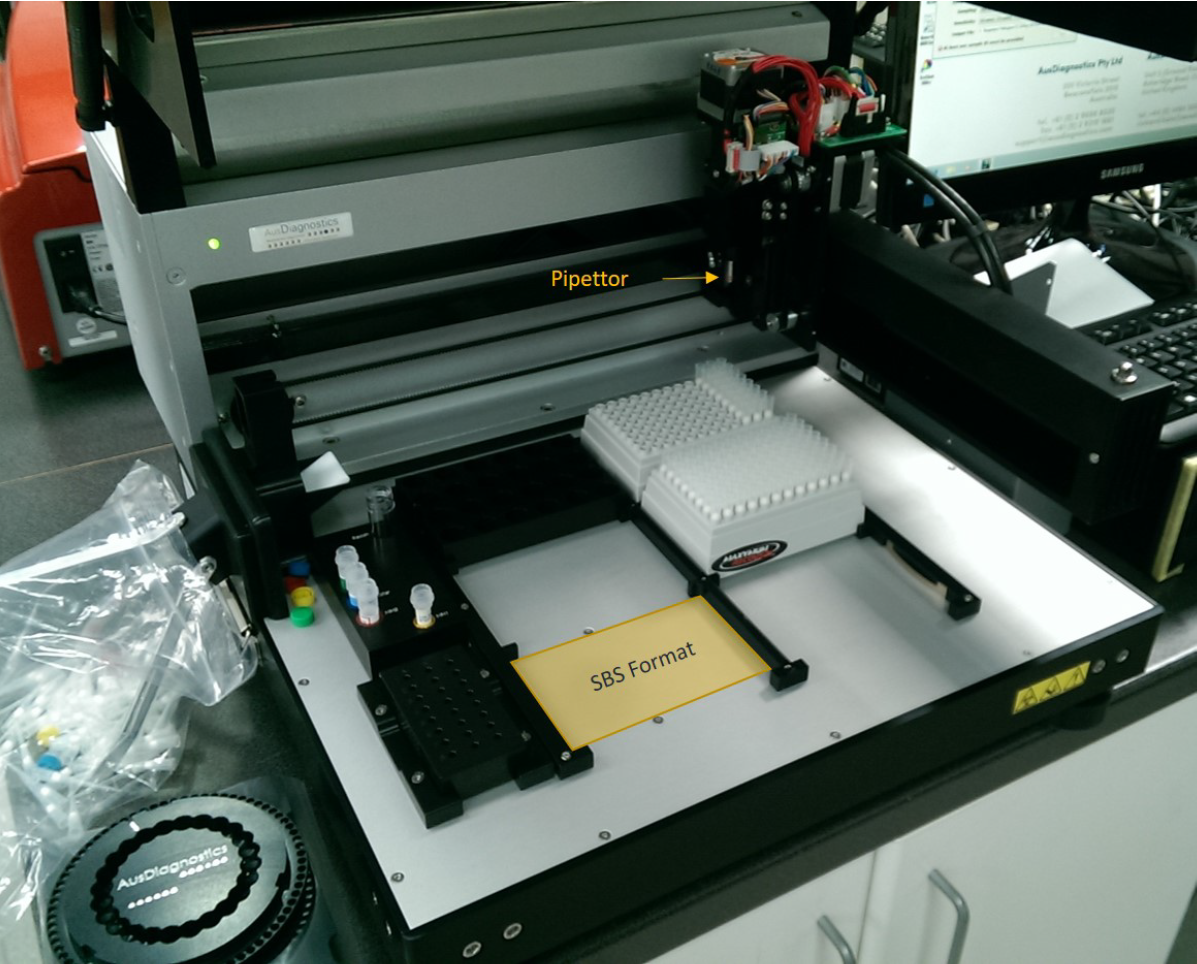
\includegraphics{highplex.png}
	\caption[High-Plex Platform.]{The Gene-Plex liquid handling robot platform, as implemented as the High-Plex Processor.}
	\label{fig:highplex}
\end{figure}ˆ 

\subsection{The Extraction Process}
\label{subsec:intro_extraction}

In order to allow the aims and scope of the work to be clearly defined, a condensed overview of the extraction process developed by AusDiagnostics is presented.

The extraction process requires that the clinical sample undergoes a number of chemical steps across different locations on the robot. To aid in understanding the liquid handling involved, Figure \ref{fig:decklayout} displays the important sites on the deck. The process will begin with the operator manually loading 24 individual clinical samples into the location labelled ``Clinical Samples". In order to conform to existing products used by customers, it is then required that the chemical processing takes place in the locations labelled ``Samples". In order to transfer the liquid between locations, the robot will pick up 1000$\mu$L tips from the locations marked ``Tips". 

The sample processing locations must accept modules that fit within the standard block size (SBS) format. In these modules, the sample will undergo the following 6 stages in order to extract the target DNA and RNA:
\begin{enumerate}
	\item 
\end{enumerate}

\begin{figure}
	\centering
	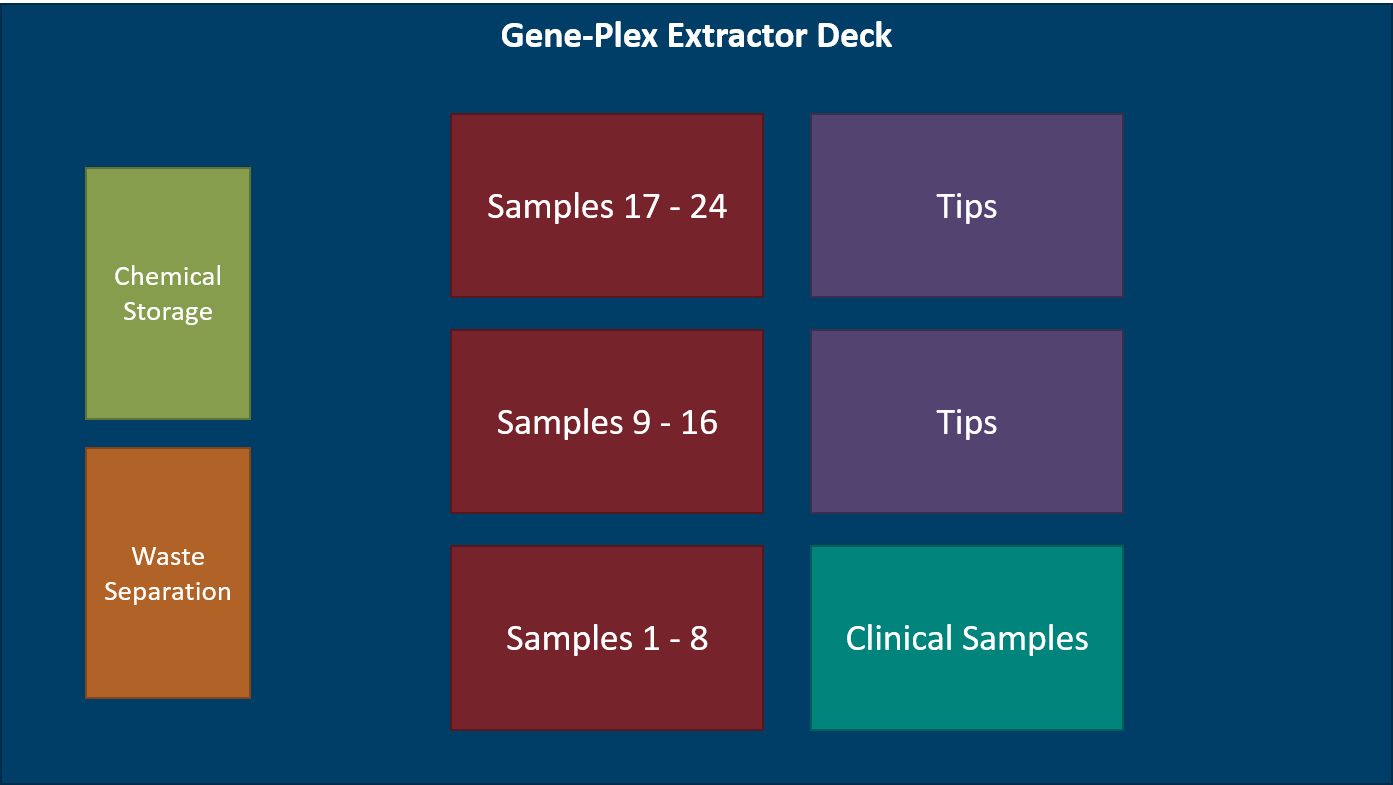
\includegraphics{decklayout.png}
	\caption[Extractor deck layout.]{The layout to be used for the Gene-Plex Extractor.}
	\label{fig:decklayout}
\end{figure}ˆ 



\section{Aim}
\label{sec:intro_aim}

\section{Scope}
\label{sec:intro_scope}

\section{Methodology}
\label{sec:intro_method}




% Figure 1.1 is defined below (Large mechatronics logo). Note figures are placed automatically by LaTeX and will not necessarily be placed before the next text.
\begin{figure}
\centering
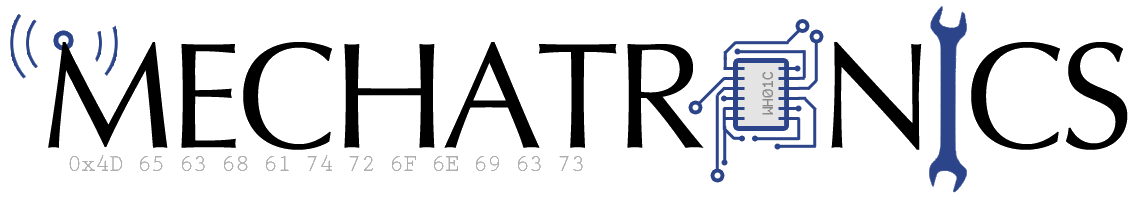
\includegraphics{mechatronicslogo2_no_UNSW.png}
\caption[Short caption for list of figures.]{Full caption for the Mechatronics Logo. Designed by Wei Hua Chen.}
\label{fig:intro_logo}
\end{figure}

\begin{figure}[!ht] \centering
\captionsetup[subfigure]{width=2.5in} % <-- Use this to control text which is poorly spaced under a subfigure. 
\begin{subfigure}[t]{0.45\textwidth}
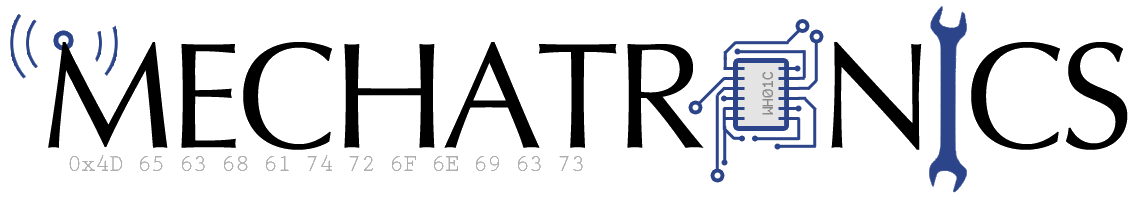
\includegraphics[width=\textwidth]{mechatronicslogo2_no_UNSW.png}
\caption[Subfigure caption.]{Subfigure caption.}
\label{fig:intro_subfig1}
\end{subfigure}
\begin{subfigure}[t]{0.45\textwidth}
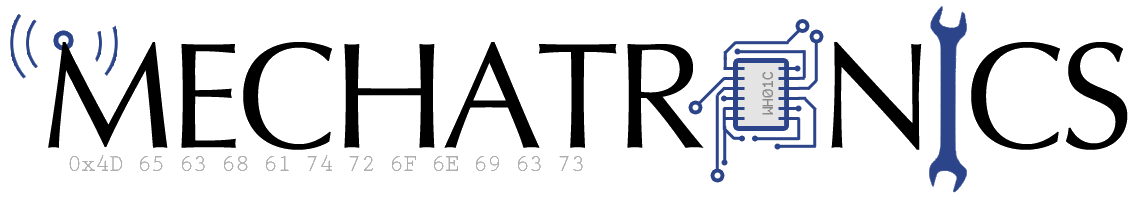
\includegraphics[width=0.5\textwidth]{mechatronicslogo2_no_UNSW.png}
\caption[Subfigure caption.]{Subfigure caption.}
\label{fig:intro_subfig2}
\end{subfigure}
\caption[Abbreviated caption.]{Overall figure caption.}
\label{fig:intro_subfig}
\end{figure}

Figure \ref{fig:intro_subfig} and subfigure \ref{fig:intro_subfig2} or \subref{fig:intro_subfig2} contains ...
Table \ref{tab:intro_table_1}. 

Citations: Luce \cite{luce_probabilistic_1958} wrote something important.

% Note: You can add a table of figures to the header pages by uncommenting \listoftables in the frontpages.tex

\begin{table}[h!]
\begin{center}
\begin{tabular}{ p{3cm}  p{4cm} | p{6.5cm} }
\hline
Classification & Cost & Description\\ \hline \hline
CLEAR & 1 & Good for traversing\\ \hline
OBSTACLES  & $\infty$ & Definitely not traversable\\ \hline
UNKNOWN & 4 if distant, $\infty$ if close & Not classified\\ \hline
EXPENSIVE & In range $[2, 50]$ & Traversable but should be avoided\\ \hline
\end{tabular}
\end{center}
\caption[Example table (short caption).]{Example table.}
\label{tab:intro_table_1}
\end{table}
\chapter{Literature Review}
\label{cha:literaturereview}

\section{Heating}

The thermal requirements for the extractor to be developed, as outlined in Chapter \ref{cha:introduction}, are very similar in nature to those of a Polymerase Chain reaction (PCR) Thermal Cycling Device, albeit with simplified operations. The requirements of a PCR thermal cycler are driven by the need to cycle the temperature of an array of tubes containing a small volume of sample liquid through temperatures of 55$\degree$C, 72$\degree$C, followed by 92$\degree$C \cite{14405884}. Due to the process involving upwards of 20 cycles between these temperature set points, ramp times for these changes in steady state must also be minimised to ensure the total processing time is commercially viable. The thermal requirements of the Gene-Plex Extractor are highly matched, with two exceptions. In this application the temperature of the sample liquid shall be held at a constant 60$\degree$C, as determined by research conducted by AusDiagnostics, as opposed to the multiple temperatures of a PCR cycler. Secondly, the cool down ramp rates for a PCR cycler are of equal importance to it's ramp rates during heating, in order to achieve temperatures lower than the current steady state in adequate times \cite{2563996}\cite{15156909}. In the application of the Gene-Plex Extractor, there is no need to pay attention to cooling ramp rates as the system will only cool at the completion of its operation. Due to the similarities evident between these two applications, a great deal of information may be gathered from PCR cycler design.\\

In order to generate the heat necessary to reach the required sample temperature, some form of thermal pump is required. A Thermoelectric Cooler (TEC), also know as a Peltier, is often used for liquid sample thermal cycling \cite{12436620} among its' many other applications. A TEC is a solid state heat pump, controlled by the directional application of electric current across it's two terminals \cite{20160801988967}. The direction of the applied current determines the direction of heat pumping across the module \cite{20160801988967}. TEC's are constructed of pellets of n-type and p-type bismuth telluride semiconductors, connected in an alternating series \cite{6464884}. The connections, made of copper, are bound to a substrate of ceramic alumina. This substrate forms the surface by which the heat generated is transferred. Figure \ref{fig:tec} displays the arrangement of a TEC in a general case application. The TEC has shown through the reviewed literature to be common in PCR thermal cycler applications due to the above mentioned ability to pump heat in either direction, allowing ramping of temperature to be precisely controlled equally in both directions.\\

\begin{figure}[!htb]
	\centering
	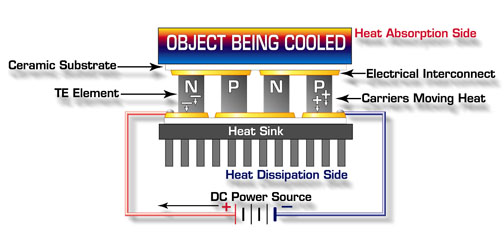
\includegraphics[width = \textwidth]{tec.jpg}
	\caption[Thermoelectric Module Application.]{Thermoelectric module as assembled in a typical application. \cite{Ferrotec}}
	\label{fig:tec}
\end{figure}ˆ 
\FloatBarrier

When used in control applications, a TEC has the advantage of being able to not only add but to also remove heat energy as is required by the controller to achieve the desired response. Despite the TEC's ability to actively remove heat from a component, other active temperature removal methods may also be implemented. A passive approach to heat removal is that employed by a heat sink, or any simple surface area \cite{2006289990179}\cite{20144600208116}. This differs from an active approach, where airflow over the heat sink surface area is controlled via a fan, for example \cite{2006289990179}. Such methods may be substituted for the directional heat pumping capabilities of the TEC, in order to achieve a similar level of temperature control. This leads to simpler possible options for heat pump selection, namely electric resistive heaters. Despite no reviewed literature describing these devices as the main heat source in thermal control for PCR in particular, they have been demonstrated to provide a crucial supporting role by Williams et al. The thermal cycler described in the work of Williams utilizes resistive heat strips to control the temperature of a sealing lid, preventing sample evaporation at the upper operating temperatures of a PCR thermal cycler \cite{7238517}. While the application noted here differs from the intended application within the extractor, where the device will be the primary source of heat, it demonstrates the feasibility of driving component temperature to a steady state value and hence represents a design possibility.\\

\section{Cooling}
In order to be able to control the temperature of the liquid sample as required, a method of evacuating heat must be present. A passive method alone, such as a heat sink in isolation, will not allow the process controller to drive a reduction in heat beyond the limits of conduction to the surrounding air \cite{20144600208116} and as such performance will not be satisfactory. Along with heat dissipation being essential for control, the TEC elements have a maximum temperature differential of which they are capable of generating across their surfaces. This imposes the following constraint on the thermal system:
\begin{equation}
T_{hot} - T_{cold} \leq dT_{max}
\end{equation}
This has been noted as highly significant in PCR cycler design \cite{20160801988967}, where one end of the TEC must be kept at ambient temperature to enable the maximum steady state value of 92$\degree$C to be reached safely. It should be noted that due to the maximum steady state temperature in this application being limited to 60$\degree$C and assuming a reasonable TEC differential limit, $dT_{max}$, this constraint is not critical. However, a TEC becomes less efficient as it's temperature differential is increased \cite{20070113880}. As such, a method of heat evacuation must be present.\\
%FOR last sentence, it is more correct to state that it is desirable to maintain a heatsink temperature at room temp to minimise differential

%NOTE: for the above explanation, include a graph of peltier temperature differential vs power transfered, as http://www.heatsink-guide.com/peltier.htm. This is in widomski.

\section{Controllability}
\label{lit_controlability}
In order to create a thermal system which is controllable within the context of stability and speed of response, attention must be paid to the thermodynamics of the device. Due to manufacturing constraints and standards, the tube which contains the sample itself is not optimal. A wall thickness of 1mm results in poor heat transfer characteristics from the heated block to the sample \cite{1704922}. Another source of poor dynamics is any regions of mechanical connection between the heated block and external components \cite{7238517}. Recommendations from the reviewed literature included the use of gasket material to limit thermal material between any surface contacts (Williams et al specifically recommends the use of ethylene propylene), along with the use of a groove extending through the majority of the thickness and hence limiting heat transfer to the mechanical connections \cite{20130415930883}\cite{20070113880}. Mechanical connections are however only one cause of significant thermal gradient within the device. Care must be taken to reduce the severity and frequency of the occurrence of these gradients to maintain stability and performance in temperature response. After heat pumping has ceased, a temperature gradient will persist for a period of time that is proportional to the square of the distance between the hot and cold locations \cite{7238517}. This has important implications for the number of sample tubes that may be heated within a single block. If the size of the sample array to be heated is too large, difficulty will be encountered achieving a uniform and stable steady state temperature \cite{7238517}. Widomski et al note that despite efforts to reduce heat loss and hence gradients around the system boundaries via methods such as insulation, the region of location of the heat source will continue to maintain a higher temperature. To counter this, it is suggested to use a rod of material with lower thermal conductivity (such as stainless steel within an aluminium block) to reduce the heat retained in this volume \cite{20070113880}.\\
%INLCUDE 	equation for time of gradient

A number of measures may also be taken directly related to the heated block itself to ensure optimal thermal response. The concepts of static local balance and static local symmetry may be applied to obtain desirable heat transfer within the medium \cite{7238517}. A state of static local balance refers to a state of constant temperature where all heat sinks are equalled by heat sources in a local area \cite{7238517}. This essentially describes a state of thermal equilibrium, where the following condition is satisfied:
\begin{equation}
Q_{in} = Q_{out}
\end{equation}
To ensure this balance is obtained, a device design should not incorporate overly effective heat sinks, without a proportional increase in the heat source capacity, and visa versa. The condition of static local symmetry requires that for a constant temperature and within a local region, the center of mass of the heat source is coincident to the center of mass of the heat sink \cite{7238517}. Satisfying this condition will ensure that a constant, steady state temperature is achievable, without the presence of a permanent temperature gradient between the two centers of mass. The selection of heated block material along with manufacturing methods may also act to improve transfer properties. Aluminium 6061 is recommended due to its purity \cite{7238517}, which aids in even heat transfer \cite{OLAFSSON1997}. It is further recommended that the heated block be manufactured via machining, due to the homogeneous structure that results. This is beneficial in reducing any temperature gradients that may occur within the heated element due to mechanically or otherwise joined components or impurities or inconstancies that exist as a result of other manufacturing methods such as casting.

\section{Temperature Sensors}
The literature reviewed has presented various differing selections of temperature sensing technologies, the most prominent of which have been thermocouples and thermistors. Despite the overlapping application, the specifications of the two technologies are significantly different. The thermocouple has a large temperature range, with measurements capable of ranging from -270$\degree$C to 1800$\degree$C compared to the limited range of thermistors of usually around -90$\degree$C to 130$\degree$C \cite{11303490}\cite{15156909}\cite{10650397}. The thermocouple and thermistor possess similar response rates along with similar accuracy, however due to the wider resistance range available, thermistors are able to achieve a high measurement resolution \cite{11303490}\cite{15156909}\cite{10650397}. The two significant differences between the technologies are power supply requirements and linearity. Due to the welding of differing metal conductors at the measuring point, the thermoelectric effect results in a temperature dependant voltage being generated across the thermocouple terminals \cite{11303490}\cite{10650397}\cite{15156909}. While this means the sensor does not require a power supply, it can introduce complications requiring a reference/compensating wire. Furthermore, changes to the conductor materials such as corrosion require that the sensor be calibrated on a regular basis, often as frequently as 3 months \cite{11303490}\cite{15156909}\cite{10650397}. Thermistors use semi-conductive material that changes resistance with temperature. As such, measuring the temperature requires a current is passed through the device \cite{11303490}\cite{15156909}. While the output voltage of thermocouples changes linearly with temperature, this is not true of thermistors. Hence, the output signal requires linearisation before it may be of use \cite{15156909}. In commercial applications, thermistor technology is often also preferred due to its cost effectiveness \cite{10650397}. While Resistive Thermal Detectors (RTD's) and Integrated Temperature Sensors appeared in a number of reviewed sources, they are not considered in depth due to the high level of signal conditioning required \cite{10650397}\cite{11303490} and the lack of observed uses in relevant thermal control applications.

\section{Temperature Sensing}
To utilize the thermal system to control the liquid sample temperature accurately, a method of obtaining a feedback signal is required. Complications exist however, due to the constraint that the sample temperature itself cannot be directly measured. Due to the thermal transfer characteristics discussed above, the placement of the sensing device is critical to the stability of the controlled substance \cite{20130415930883}. Vilchiz et al studied the issues of sensor hardware placement and provided numerous recommendations to increase baseline stability. Using experimental methods, it was verified that the following one-dimensional heat equation holds:
\begin{equation}\label{time lag}
s=\frac{L}{a}
\end{equation}
Where $s$ is the time taken for energy to flow from location A to location B, $L$ is the distance between the two locations, and $a$ is the thermal diffusivity of the material. This is relevant as it allows the time lag between a controlled heating action at the heat source to the arrival of the generated heat at the location of interest to be determined. The experiment conducted tested two temperature sensing cases. One sensor was placed within the center of mass of the heated block, while the other was located as close as was possible to the heat source. The results obtained found that ``there is a general advantage of control via sensing close to the heater, whether by temperature measurement, or by heat-flow control sensing.'' \cite{20130415930883}. Equation \ref{time lag} is accountable for this result. When the sensor is placed at a greater distance to the heat source, the control effort is determined using a measurement that is not yet equalised due to the more severe temperature gradient. This error in feedback signal is reduced by the recommended placement strategy, such that ``the reduction in the magnitude of the heater-induced oscillations achieved by this control strategy is at least one order of magnitude better than that of the temperature control at the core'' \cite{20130415930883}.\\
%FOR above quote, either show figure of this repsonse (ideal) or make note that response oscillated

A number of aspects of the experiments and findings the work of Wilchiz et al should however be considered. The sensing device used to make the presented conclusions were thermocouples, one of many sensing devices available. Despite the variances in accuracy and stability of measurements that are expected between differing sensing technologies, the results can be assumed independent of any associated error. Any error as a result of sensor output stability is of an insignificant order to magnitude of time when compared to the 1.07 min thermal lag situation generated by the experiment. Furthermore, one would expect a sensor technology of differing accuracy to produce a controlled output different to the desired reference input. This error is however not influential to the results given, which are concerned exclusively with the stability of the controlled response. The focus of the experiment was the application of thermocouple technology in Tian-Calvet microcalorimeter devices. This does not detract from the relevance of the reviewed work for a number of reasons. The motivation for the study was to improve baseline stability in temperature control, via the application of improved temperature measurement strategies; a general outcome that is relevant to the work of this thesis. Further to this, the scale of the experiment conducted closely resembles the device to be developed, with the distance between sensor locations set equal to 3.5cm. Therefore, despite the differing applications of the work conducted, the recommendations and strategies found may be concluded as directly applicable.

\section{Controller Design}
With the necessary hardware in place and optimally set up, as has been discussed above, controller design and theory may be considered. The large majority of the reviewed literature, along with the instruments currently employed by AusDiagnostics, recommend or employ the Proportional Integral Derivative (PID) controller. As summarised by Vilchiz et al, ``Although other types of controllers are also feasible, e.g., those based on fuzzy logic or artificial neural networks, the simplicity, good response, and low cost of PID-based control loops have motivated their popularity in industrial applications'' \cite{20130415930883}\cite{20160801988967}. Despite the common application of the PID controller in thermal control applications, if a TEC is the selected source of heat, complications are presented. Due to the non-linearity of the device, PID coefficient selection involves the process of trial and error \cite{20160801988967}. The strategies for PID design given were however applied to the thermal cycling requirements of PCR. This requires that 3 separate temperature controllers be implemented for each of the temperature set points, to ensure the required performance is met equally at each \cite{20160801988967}. While the characteristics of the PID controller are not effected by this difference, it does significantly increase the complications of coefficient selection in comparision to the application in the Gene-Plex Extractor. Further to the controller to be implemented itself, a number of sources give recommendations regarding relevant hardware. Cellatoglu et al investigated the dynamic performance of a process control system, with a focus on temperature controllers. The findings reveal that the word length of the ADC utilised is an important factor in reducing output error. A case study was conducted to assess the impact of increased word length on error, with results suggesting that 8 bits is the optimal value \cite{12096602}. It was further found that an increase in word length beyond this point yields no reduction in error. The analysis conducted was however completed as a simulation, with no experimental verification evident. The electronic hardware implemented in other sources, such as the work of Shirafkan et al, differs from this recommendation. While  not providing evidence to suggest the 8-bit recommendation is problematic, the successfully implemented controller utilized a 24-bit ADC.\\

%NOTE: fIGURE FOR ADC WORD LENGTH?
\section{Magnetic Separation}
To ensure the target DNA is extracted as required, the device must include a robust means of capturing the magnetic beads. Despite offering an alternative means of magnetic bead manipulation, electromagnets are not investigated for application in the thesis due to a high level of complexity that is not required for this static, constant force implementation. Therefore, the review of literature focuses on permanent magnets. While there are numerous compositions of magnets available, the rare earth variety and in particular the Neodymium composition (ND-Fe-B) are most suitable. Neodymium magnets offer the strongest solution, with an energy product of up to 56 MGOe \cite{2006189852255}. Good mechanical characteristics and energy to size ratio make them suitable for fastening within a manufactured product, without undue difficulty. Importantly, given the requirement to capture beads within the heated block element, Neodymium magnets are stable in temperatures near ambient. Progressive loss of magnetism occurs at temperatures greater than 80$\degree$C \cite{2006189852255}, providing a 20$\degree$C margin of safety between the operating temperature of 60$\degree$C. This composition also holds a very high coercive force \cite{2006189852255}, allowing it to resist demagnetisation in the presence of external magnetic fields that will be present within the Gene-Plex Extractor, as a result of other hardware. Despite the specification of the superparamagnetic silica beads being a constraint determined by completed research at AusDiagnostics, a number of characteristics should be noted in order to obtain reliable bead capture capabilities. Shevkoplyas et al describes the force acting on a superparamagnetic bead due to an applied force. The context of this paper is the motion prescribed by the beads within a microfuidic chamber, however the general characteristics of the interaction between the beads and magnetic field are applicable to the capture required here. In order to saturate a suspension of superparamagnetic beads, an external magnetic field greater than 0.5T must be applied \cite{9774403}. Saturation is the state where all beads' magnetic poles are aligned. In a state of saturation, the magnetic beads behave simply as permanent magnets \cite{9774403}\cite{8667402}. In order to ensure the complete separation of the magnetic bead dispersion within the sample liquid, this condition must be achieved.\\
% NEED to elaborate on magnetic capture. Also give equations and figures to show.

The literature reviewed has allowed a number of critical elements of thermal control and magnetic separation, being the main requirements of the extraction system, to be recognised and evaluated within the context of this thesis. The similarity between the processes demanded by the extraction technique and the works discussed allow the information gathered to be applied directly to the benefit of the developed instrument. Those works which were an exception to this allowed general strategies and design characteristics to be collected, which may be applied with consideration in future development.

%NOTE: NEED TO INCLUDE SOME HALBACH ARRAY
\chapter{Methodology}
\label{cha:methodology}

With the scope of the work now defined, the manner in which the required results will be obtained can now be detailed. The necessary additions as defined in Section \ref*{sec:intro_scope}, Scope, may will be implemented in the form of two independent assemblies in order to meet the requirements of the work. These two assemblies will be refereed to as the Processor Module and the Magnetic Separation Station. The former will be the site of the chemical reactions as described in Section \ref{subsec:intro_extraction}, The Extraction Process, and will be the hardware element that forms the SBS block on the Gene-Plex Extractor deck. Therefore, given it will house the full set of reactions, it will also encompass the software and hardware requirements of the liquid temperature control (including the associated controller), along with the magnetic separation required in tube number 4 of the cassette. The Magnetic Separation Station will be the location of disposal of the supernatant and therefore shall include the magnetic hardware required to physically manipulate the magnetic silica beads in order to retain them in the pipette tip while the waste is expelled. Given the biological nature of the liquid waste involved, this station will also include provisions for hygienically disposing of and storing this waste.

\section{Processor Module}

\subsection{Hardware}

%NOTE : need to atleast mention use of autodesk CFD and rough method

The hardware component of the Processor Module design is concerned with ensuring the module accepts the required cassette tubes, fits within the stipulated SBS space and provides a stable platform for the required temperature control using the knowledge gained in Section \ref{lit_controlability}, Controllability. The work in this sections will also include the selection of an appropriate heat pumping device. In order to ensure the requirements of the hardware elements are met, the design process is applied as follows:
\begin{enumerate}
	\item Generation of concepts related to thermally isolating the heated and non-heated regions of the block. This includes a focus on the manufacturability of the resulting components.
	\item Investigation into and selection of an appropriate heating method.
	\item Full CAD design of hardware including provisions to accommodate the required tubes.
	\item Utilization of 3D printing to test the fit of the cassette tubes in the block design.
	\item CFD simulation to verify the performance of the selected heating element and the thermal stability of the final design. 
\end{enumerate}

\subsection{Temperature Controller}

This work will result in the finalisation of a software temperature controller capable meeting the liquid heating requirements of the chemical reaction as detailed in Section \ref{subsec:intro_extraction}, The Extraction Process.

In order to enable controller design to be commenced, the first step will be to assemble the completed Processor Module. Due to the complex dynamics of the heat transfer between the heating device and the liquid, a mathematical modelling method is not used. Instead, the system will be identified via the step input response plant identification method. To obtain the required response data, sensors will be placed strategically on the Processor Module to monitor and record key temperatures:
\begin{itemize}
	\item The temperature at the centre of the block will be taken as this sensor data will be utilized as feedback for the controller to be implemented. This follows the recommendations given in Section \ref{cha:literaturereview} by Vilchiz et. al.
	\item The temperature of the heatsink will be plotted to monitor the temperature differential created across the module.
	\item The temperature of the heated region of the module will be taken on its outer surface to determine the success of the design in creating a component that responds to temperature control in responsive and stable manner.
	\item The temperature of the liquid within the cassette tubes will be measured as the final output of the system. The ability of the controller to drive this temperature to the desired set point will determine the success of the design.
\end{itemize}

To utilize this data for experimental plant identification, an Arduino will be used as an interface between the sensor electronics and MATLAB. This will enable the real-time monitoring and plotting of the data along with storage and subsequent analysis through the Arduino's Analogue input ports.\\

With the hardware now setup, the Processor Module will then be excited by a step input. The input will be provided by the same controlling electronics used in the final Processor Module. As was detailed in Section \ref{sec:intro_scope}, Scope, the companies MTX Cycler electronics driver board will be utilized. The software controlling this board will therefore be modified to provide a constant step input to the Processor Module. The step input will be applied and the response data logged until a steady state has been achieved.\\

This data will have been logged in the MATLAB workspace in real-time, during the experiment. Prior to analysis however, the data will be pre-processed to remove any unnecessary features. For example, the data will be seroed so that the response data begins at time $t = 0$ and so that the response begins at $0\degree$C. This will remove any effects of the varying room temperature at which the experiment may occur and ease the fitting of curves to the collected data.\\

To complete the plant analysis process using the pre-processed data, the MATLAB PID Tuner tool will be used. This tool provides a GUI for specifying a set of response data, the step input provided. This information is then used to interactively fit an appropriate function to the plants response data. The tool offers a number of plant structures to allow the correct plant to be identified. These range from a simple "One Pole" plant to a discrete time system.\\

As a result of this process, the transfer function which represents the plant of the Processor Module will be known. This plant will be in the continuous time domain and is represented by:

$$G_p(S)$$

Before utilizing the identified plant for controller design, it will be verified via simulation in Simulink. The validation will be conducted by providing the plant an identical step input as was done experimentally and verifying that the responses match. The Simulink layout used to conduct this simulated verification is shown below in Figure \ref{fig:openloopplant}.\\

\begin{figure}[!htb]
	\centering
	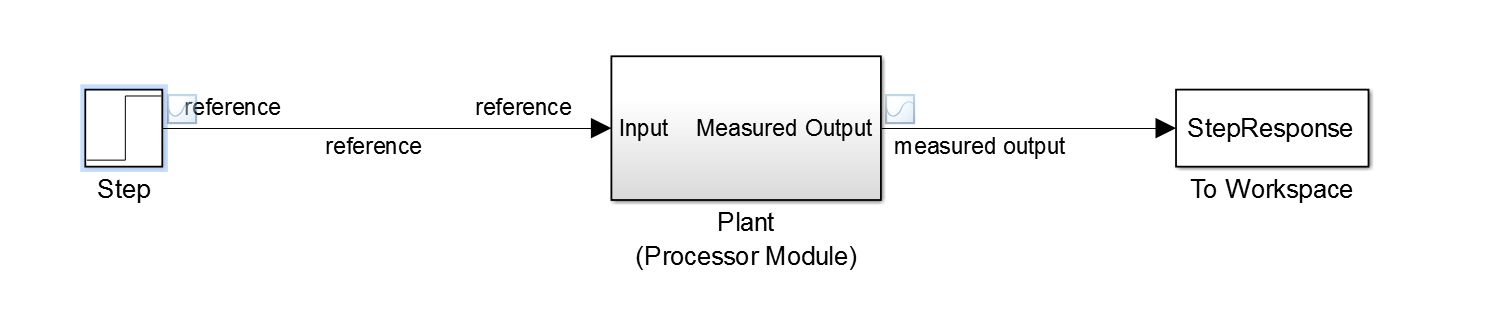
\includegraphics[width = \textwidth]{openloopplant.png}
	\caption[Open loop plant valiation Simulink Model.]{The Simulink model layout used to validate via simulation the identified plant for the Processor Module.}
	\label{fig:openloopplant}
\end{figure}ˆ 
\FloatBarrier

With the transfer function representing the Processor Module now known, the process of controller design may be commenced. The method chosen for this design process is the Direct Analytical Method (also known as Ragazzini's Method), in the discrete time domain. As was noted in Chapter \ref{cha:literaturereview}, Literature Review, the most common method of control for thermal cycling devices in similar applications is PID control. This method has not been selected however due the benefits of competing controller design in the z-domain with discrete time. By completing the design entirely in the z-domain, there is no need to convert the resulting controller from the s domain, allowing the controller to be directly implemented.\\

The direct analytical method uses the principle that if the output that is required along with the input applied is known the intermediate transfer function may be determined. This is represented by Equation \ref{eq_direct}, where $C(z)$ is the required output, $U(z)$ is the applied input and $F(z)$ is the intermediate transfer function.

\begin{equation}
\label{eq_direct}
C(z) = F(z)U(z)
\end{equation}

The method of feedback used for the controller is a unity feedback signal. Data provided by the utilized sensor will be processed to give a feedback signal with unity gain, to ensure any features of the raw signal are removed. For the unity feedback system picture in Figure \ref{fig:unityfeedback}, $F(z)$ is given as \cite{UNSW}:

\begin{equation}
F(z) = \frac{G_c(z)G_p(z)}{1+G_c(z)G_p(z)}
\end{equation}

\begin{figure}[!htb]
	\centering
	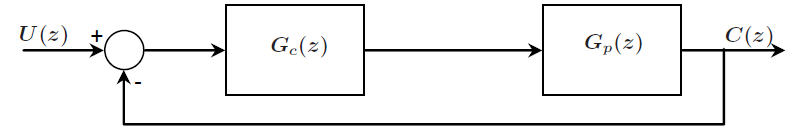
\includegraphics[width = \textwidth]{unityfeedback.png}
	\caption[Unity feedback system.]{The block diagram for a unity feedback system. \cite{UNSW}}
	\label{fig:unityfeedback}
\end{figure}ˆ 
\FloatBarrier

Due to the plant identification completed earlier, the continuous time form of the system plant is known. Using MATLAB, this may be converted to a discrete time transfer function, with the appropriate sampling time selected. Therefore, $G_p(z)$ is known.\\

Rearranging for the controller of interest, $G_c(z)$ gives:
\begin{equation}
\label{eq_controller}
G_c(z) = \frac{F(z)}{G_p(z)[1-F(z)]}
\end{equation}

By equation \ref{eq_controller}, the direct method requires only that $F(z)$ be determined to realise the controller. To complete the formation of $F(z)$ and hence $G_c(z)$, the method below will be utilized. This method, as detailed by J. Katupitiya \cite{UNSW}, provides a number of steps to ensure the resulting controller performs as required.\\

\subsubsection{Controller Performance}

To define the response time of the controller, the pole locations are set. To do so, the desired time constant of the system, $\tau$ is set and the s domain pole is found by:

\begin{equation}
s = -\frac{1}{\tau}
\end{equation}

This s domain pole is then transferred to the z domain via:

\begin{equation}
z = e^{sT}
\end{equation}

Where T is the sample time of the controller. The resulting pole is then placed as a pole of $F(z)$.\\

It is also important to control the steady state error of the controller. To do this, the DC gain of the system is set to 1, resulting in the output equalling the input at steady state. By setting the following, this can be achieved:

\begin{equation}
F(z)|_{z=1} = F(1) = 1
\end{equation}

\subsubsection{Pole Zero Cancellation}

It must be ensured that a pole or zero cancellation does not occur in the unstable region of the Z-Plane, in order to ensure that this cancelled pole does not become a component of the formed characteristic equation. If a controller component cancels an unstable plant pole or zero in this scenario, it will influence the system so that it becomes unstable. These constraints will be dealt with via two stability constraints:\\

\textbf{Stability Constraint 1}\\
Stability constraint 1 addresses the instability that may occur if a pole of the plant $G_p(z)$ is cancelled by a zero of $G_c(z)$. Firstly, all poles of $G_c(z)$ are tested for instability, where any pole $z = p_0$ is unstable if :

\begin{equation}
\label{eq_unstablepole}
|p_0| > 1
\end{equation}

If any pole is found to satisfy Equation \ref{eq_unstablepole}, it is unstable and must be added as a zero of $[1 - F(z)]$. This addition removed the unstable pole and ensures the controller is not able to create the unstable cancellation.\\

\textbf{Stability Constraint 2}

Stability Constraint 2 deals with the case that an unstable zero exists in the plant transfer function. Therefore, it prevents a pole of the controller from cancelling this zero in the unstable region. A zero of the controller $G_c(z)$, $(z = z_0$ may be tested for instability by checking if it satisfies Equation \ref{eq_unstablezero}:

\begin{equation}
\label{eq_unstablezero}
|z_0| > 1
\end{equation}

Any zero satisfying this equation can be identified as unstable and dealt with by including it as a zero of $F(z)$.\\

\textbf{Causality Constraint}

The causality constraint ensures that the designed controller is either proper or strictly proper. That is, that it only uses current or past terms in the calculation of controller effort and no futuristic terms. This is achieved by ensuring the pole-zero deficiency of the plant (i.e. its delay) is either that same as or less than that of $F(z)$. The pole-zero deficiency of he plant is the order of the denominator minus the order of the numerator, denoted as:

\begin{equation}
\label{eq_plantdef}
D[ G_p(z) ] = n
\end{equation}

The pole zero deficiency of $F(z)$ is given as:

\begin{equation}
\label{eq_fdef}
D[ F(z) ] = m
\end{equation}

If $m = n$, the controller is strictly proper. If $m > n$, the controller is proper. However, if $m < n$, then the controller is improper (will require futuristic terms) and the causality constraint is not satisfied. In this situation, the order of the denominator of $F(z)$ must be increased until the controller is at least strictly proper.\\

\textbf{Controller Difference Function}

Using the $F(z)$ found using the previous steps, the controller transfer function, $G_c(z)$ can then be calculated. This transfer function is converted into a function of the variable $Z^{-1}$, which is commonly known as the Digital Signal Processing (DSP) format. This allows the transfer function to be directly written as a difference function involving multiple error and controller effort terms with varying time delays. This difference function is the realised discrete controller.\\

\textbf{Simulated Validation}

In order to validate the design of the controller prior to implementation, the design will be simulated via Simulink to validate its response to the desired reference input. The block diagram shown in Figure \ref{fig:controllervalidation} will be used to conduct the validation and record the resulting data. The response recorded will be assessed against the controller requirements.

\begin{figure}[!htb]
	\centering
	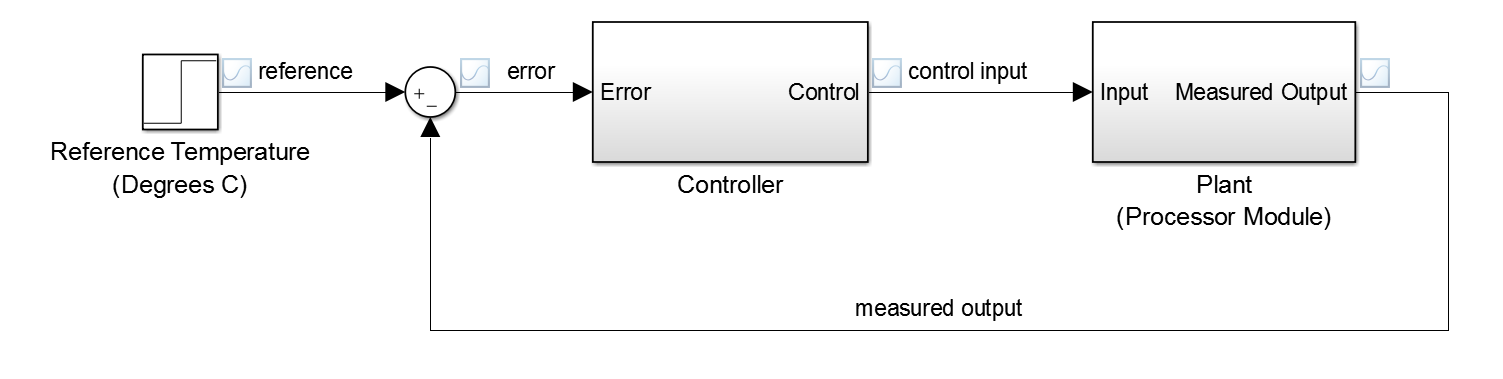
\includegraphics[width = \textwidth]{controllervalidation.png}
	\caption[Controller valiation Simulink Model.]{The Simulink model layout used to validate via simulation the designed controller for the Processor Module.}
	\label{fig:controllervalidation}
\end{figure}ˆ 
\FloatBarrier

Following the successful validation of the temperature controller, it will be implemented via software currently driving the MTX cycler, along with any required modifications.

%UP TO HERE

\subsubsection{Experimental Verification}

In order to verify the performance of the resulting controller, the following experimental verification will be conducted. The experiment will determine the ability of the controller to meet the steady state error, disturbance rejection, response time, overshoot and stability requirements when controlling temperature in the module. The method is as follows:

\begin{enumerate}
	\item Assemble 4 complete Processor Modules
	\item Using an Arduino as an interface and MATLAB as the data logger and analyser, measure the temperature in the tubes shown in Figure \ref{fig:measuredtubes} for the duration of the experiment.This distribution will allow the performance at the extremes of the device to be determined.
	\begin{figure}[!htb]
		\centering
		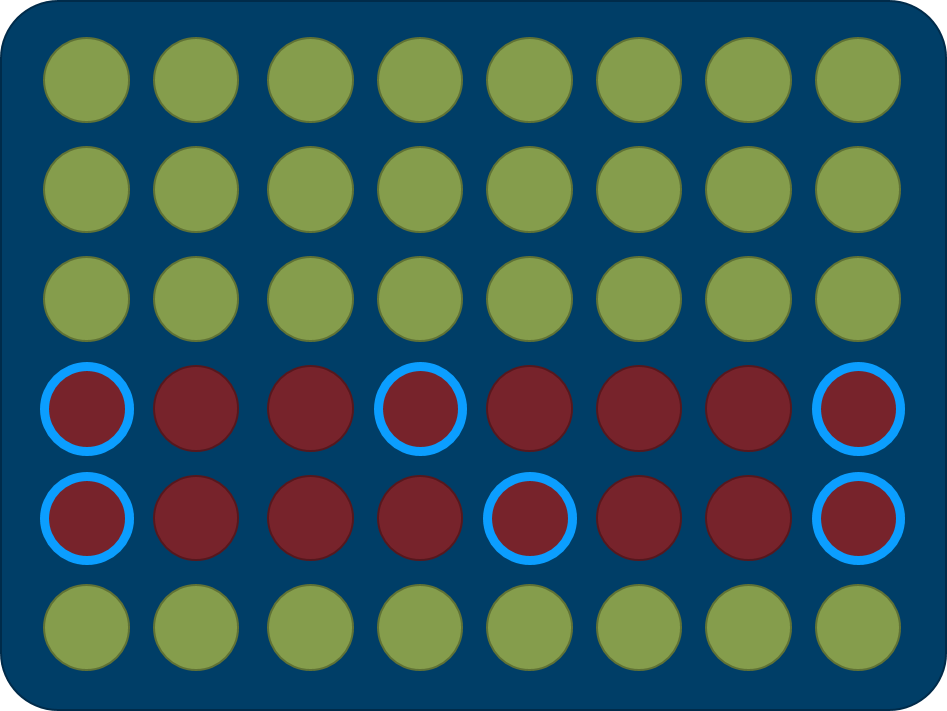
\includegraphics[width = \textwidth]{measuredtubes.png}
		\caption[Temperature Measured Tubes.]{Tube locations to be measured during temperature control verifications experiment. Non-Heated tubes are coloured green, heated tubes are coloured red, measured tubes are outlined in blue.}
		\label{fig:measuredtubes}
	\end{figure}ˆ 
	\FloatBarrier
	\item Begin data logging and live plotting.
	\item Set the reference input to the controller to 60$\degree$C.
	\item Collect data for a total of 30 minutes to capture the long term steady state performance of the module (to allow any slow heat transfers to be observed) along with the transient response.
	\item Repeat the experiment for all four assembled modules. This allows for the controllers ability to reject disturbances caused by the differing of the plant properties to be determined as is caused by the slight differences in assembly.
	\item Repeat experiment in differing environmental conditions. The experiment should  be conducted in rooms at temperatures of 18$\degree$C, 22$\degree$C and 26$\degree$C. This allows for the disturbance rejection of the controller to be assessed where the disturbance is due to altered environmental conditions.
	\item Use the collected data to assess the consistency of the heating profile and the temperature stabilisation across the tubes of the module. These results will be used to make conclusions regarding the designed controller along with the thermal characteristics of the hardware. It should be noted that the worst case response will be used to draw conclusions regarding performance to ensure all samples fall within the requirements.
\end{enumerate}

\subsection{Magnetic Separation}

As the final stage of the extraction process is the removal of the clean sample from the waste beads, the success of extraction depends on the complete and reliable separation in tube number 4. To ensure this is achieved, the following design process and experimental verification will be conducted:
\begin{enumerate}
	\item An investigation will be conducted into the various possible methods of magnetic separation in this application, taking into account the recommendations to use ND-Fe-B magnet compositions as found in the reviewed literature.
	\item 3D Printed test jigs will be created to test the effectiveness of the most suitable configurations via manual inspection.
	\item With a preferred design selected, the a test module will be 3D printed including the magnetic arrangement. This test module will be assembled on the robot deck and verified experimentaly via the method described below.
\end{enumerate}

\subsubsection{Experimental Verification}

To allow a confident conclusion to be made regarding the effectiveness of the magnetic separation within the Processor Module to be made, the following experiment will be conducted. This experiment will replicate the setup used by the robot and its processes to ensure the result is representative of the true scenario.

\begin{enumerate}
	\item Place test module with magnetic separation on Gene-Plex Extractor deck within one of the SBS spaces.
	\item Place a 5mL tube on the robot deck to collect the experiment output.
	\item Place a full set of 8 cassettes in the test module with 100$\mu$L of filtered water and 10$\mu$L of magnetic beads in tube 3. The water will simulate the elution buffer. Both volumes are equal to that used in the final process.
	\item Instruct the robot to aspirate the mixture in tube 3 and expel it into tube 4, the location of the magnetic separation.
	\item Wait for 5 seconds for separation to take place. It should be noted that this waiting period is a design variable and may be adjusted and this experiment repeated to determine the optimal wait time.
	\item Aspirate the separated liquid at a distance of 1mm from the tube bottom. This distance once again may be adjusted, however is a sound starting point for experimentation.
	\item Expel the liquid from the tip into the 5mL tube on the deck.
	\item Repeat this separation procedure for all 8 cassettes.
	\item Refill all cassettes with equal volumes of water and beads, as was defined in step 3.
	\item Repeat the separation for a total of 3 modules to equal the total volume of liquid which will be processed by the Gene-Plex Extractor during the processing of all 24 samples.
	\item Place the 5mL tube with extracted contents adjacent to a large ND-Fe-B magnet to draw any beads to the tube wall. Examine the tube contents for any sign of magnetic beads. The presence of a bead within the tube indicated a failed separation within tube 4. Such a result may lead to severe complications in step 2 (amplification), such as the failed diagnosis of a patient. Therefore, for a successful verification, it is required that no beads are present.
\end{enumerate}

\section{Magnetic Separation Station}

The magnetic separation station is a standalone module on the robot deck which will fulfil two requirements of the extraction process. Firstly, the station will provide the means of separating the waste liquid from the magnetic beads and captured DNA/RNA, as necessary after step 2 (refer to Section \ref{subsec:intro_extraction}) of the extraction process. Following the successful separation of the supernatant, the separation station will provide a means of hygienically disposing of the associated biological waste. The work will be completed via the the methodology described below.

\subsection{Magnetic Separation}

This stage of the extraction process carries a high level of significance in relation to the final result. Poor magnetic separation may effect the reliability of the diagnosis due to a reduction in the sensitivity of the step 2 amplification, or failure of step 3 analysis due to the presence of inhibitors. The former may be caused by a lack of concentration of the target DNA or RNA in the extracted clean sample. Failed magnetic separation could cause this by not properly capturing the magnetic beads and bound target, allowing them to be expelled into waste. This loss of target will lower the sensitivity of the amplifications stage and hence may lower the accuracy of diagnosis. The second scenario of inhibitors may occur if some of the waste liquid remains after washing, contaminating the sample and lowering the effectiveness of the amplification and analysis steps. Therefore, the method used for the design of the magnetic separation capabilities of the Magnetic Separation Station is aimed at ensuring a strong and reliable separation.

\begin{enumerate}
	\item An investigation will be carried out to determine the most suitable magnetic arrangement for providing reliable separation. Similar to the treatment of the magnetic separation capabilities within the Processor Module, the investigation will focus on those employing the ND-Fe-B composition.
	\item The selected configuration will then be implemented as a design concept and a CAD model generated. This detailed design will also account for a number of secondary requirements. These include maintaining a minimum distance between the pipette tip and the Separation Station at all points to remove the possibility of cross contamination occurring through liquid transfer.
	\item The detailed design will then be prototyped using 3D printing to allow experimental verification.
	\item The prototype Separation Station will then be assembled on the Gene-Plex Extractor deck along with the necessary tubes to perform magnetic separation via the experimental procedure detailed below.
\end{enumerate}

\subsubsection{Experimental Verification}

In order to verify the required performance is achieved by the designed Magnetic Separation Station, the following experiment will be performed.

\begin{enumerate}
	\item The prototyped Magnetic Separation Station will be fully assembled and positioned on the deck of the Gene-Plex Extractor.
	\item 3 cassettes and therefore 24 tubes will be positoned on the deck with 640$\mu$L of water and 10$\mu$L of magnetic silica beads in each. These volumes are equal to those used in the extraction process and this will be repeated 24 times, once for each of the 24 samples. Therefore, this setup matches the volumes to be processed by the implemented extractor.
	\item The robot will then be setup to aspirate the liquid mixture from one of the tubes.
	\item The pipette will then be positioned within the magnetic separation station and lowered to full depth. 
	%NOTE THAT A DIAGRAM OF THIS WOULD BE GOOD to show positions
	\item The pipette tip will then be raised and lowered with the full liquid height passing along the magnetic arrangment a total of 2 times.
	%DETERMINE THESE DISTANCES AND PUT IN DIAGRAM
	\item With the beads now separated from the liquid and captured on the pipette wall, the water will be ejected into the waste disposal system. For this experiment, the waste disposal will be replaced by a small glass container that may be used to collect and analyse the ejected liquid.
	\item This procedure will then be repeated for all 24 ``samples".
	\item The contents of the waste container will then be subjected to a magnetic field to collect any beads which were not correctly separated by the process. The presence of any bead within the waste liquid indicated a failed separation.
	%ADD PERCENTAGE TOLERANCES OR VOLUMES 
\end{enumerate}

\subsection{Waste Disposal}

The work on this component of the Magnetic Separation Station is concerned with ensuring the product meets key standards and requirements in order to dispose of the biological waste in a hygienic manner. The disposal of the waste generated by the process is a key factor in ensuring a successful sample extraction. Any failure to safely dispose of this waste may introduce the risk of a cross contamination occurring between two independent samples and therefore a failure to correctly diagnose the patient.\\

To ensure the waste disposal system negates these risks, the process used will focus on researching the related standards initially in order to determine the best practices which must, by regulation, be adhered to. This research will be supplemented by end user feedback. To gain this, a group of key product users will be consulted on preferred methods of waste disposal and hygiene to guide the design process. Using the results of this investigation, the design process will be used to form a final design which takes into account the gathered information and requirements and therefore produce a functional and hygienic waste disposal system.
\chapter{Results}
\label{cha:results}
% This chapter should display the results of your experiments. It should be entirely
% factual, so leave the discussion you draw from it for the Discussion chapter.
%
% You may choose to structure your thesis slightly differently, but the overall 
% approach should be the same.
%
% 1. By now you should have already described your methodology and  evaluation 
%    procedures. There is no reason to discuss these in the results.
% 2. Do not include raw data in the results chapter, leave it for the appendix 
%    or simply don't include it. If you don't think people will refer to it it's
%    probably not worth including.
% 3. Display your results in an informative way. Charts, tables, summaries, etc.
%
% If your results form a complete chapter you can use the conclusion section to
% state how the results answer your hypothesis. If you don't have a spearate
% conclusion chapter make sure you answer the hypothesis as you go. The reader
% should have answers to these before the Discussion.




\chapter{Discussion}
\label{cha:discussion}

% The discussion is where you really use your intuition to explain the results.
%
% At this stage it's usually a good idea to read through your thesis from the 
% start and check everything flows logically. Check each chapter has a strong
% introduction and conclusion. This will reinforce in your mind what you are
% doing.
%
% I like to think of the discussion as doing four things:
% 1. Structure and summarise your results into key points. And then for each...
% 2. Explain what happened
% 3. Discuss why this happened
% 4. Lead the reader toward why this significant / what this means
%
% In your conclusions you will draw from each of these points.
%
% Evans & Gruba [1] acknowledge that the discussion is a particularly hard chapter
% to start writing. They present a 4-step method to help you out.
% 1. List all the things you know that you didn't know when you started. This
%    should be a long list and doesn't have to answer the aim or have any 
%    form of structure. General ideas, snippets of knowledge, insights, things
%    that went wrong, anything!
% 2. Group these things in a rational, stuctured way
% 3. Give each group a name. This formalises it's purpose and you can use it
%    as a section heading if you like.
% 4. Structure the ideas within each group in a logical way. Reject any which
%    you don't think are beneficial at this stage.
%
% [1] Evans, D., Gruba, P. & Zobel, J., 2011. How to Write a Better Thesis, Melbourne University Press.

\chapter{Conclusions}
\label{cha:conclusions}
% If you have not read the notes for how to write a discussion I recommend
% understanding those first. The conclusion follows on directly from there.
%
% Your conclusion should make two key links.
%    1. It should answer the aim you set in the introduction chapter
%    2. It should arise from your discussion chapter
%
% You have formulated and discussed key points in the discussion, and lead
% the reader toward why they are significant. Now you can make a conclusion
% from each of these points.
%
% The folowing are some general guidelines. Depending on the structure these
% may become a bit fuzzy. I think this will especially be the case with undergrad
% thesis as we have no idea what we're doing at the start and our aim develps
% over the year.
%  - You should draw conclusions soley from the discussion chapter
%  - There should be no discussion in the conclusion chapter
%  - The conclusions should respond to the aim in the introduction
%  - Summaries are NOT conclusions. If you are summarising you are either not
%    responding to the aim or your aim is too vague.
%       Summaries are brief account of what you found, conclusions are a
%       statement of the significance of what you found - what you concluded.
%  - Conclusions should be short and concise. 2-3 pages is enough.
\chapter{Future Work}
\label{cha:futurework}

In order to complete the full set of required capabilities for the commercial viability of the Gene-Plex Extractor, as outlined in Chapter \ref{cha:introduction}, this work shall be furthered. This includes the full development of the magnetic separation capabilities and their verification, the implementation of a hygeinic waste disposal method and the addition of the required routines to the platforms software.\\

Further to this, further work is required in order to fully realise the implemented discrete time controller. Such work includes the full debugging of the developed control routine in order to identify the source of the currently experienced data overflow. Following successful debugging, the fully implemented controller must be validated using an experimental setup identical to that employed in Section \ref{sec:controller_verification}. This must be conducted to ensure the response of the controller achieves the required system performance and the transient response is as expected from the Simulink simulation conducted.

% % % Bibliography
\addcontentsline{toc}{chapter}{\numberline{}References}
\bibliographystyle{unsrt}
% Style nar gives appreviations for author first names, and also unsorted, so numbers are in order of appearance in the text.
% unsrt only gives ccorrect ordering
% abbrv only abbreviates authors first names and journal titles.
% XXX Solve bib problem - titles not shown. Try IEEETrans style file. Style 'nar' doesn't show titles.
\bibliography{../Bibtex/library} % bibtex (.bib) file location (Mendeley can create this)

% Appendix
\appendix
\chapter{Raw Results}
\label{cha:appendix}

% Here's an example of how to rotate the page so you can fit large tables
%
%\begin{landscape}
%\begin{table}[h!] 
%\begin{center} \begin{tabular}{rrrrr}\hline 
%Q & W & E & R & T \\ \hline 
%AAAAAAAAAAAAAAA & 111111111111111 & 222222222222222 & 333333333333333 & 444444444444444 \\ 
%BBBBBBBBBBBBBBB & 555555555555555 & 666666666666666 & 777777777777777 & 888888888888888 \\ \hline 
%\end{tabular} \end{center}
%\caption[Short Name]{Longer name} 
%\label{tab:appendix_tablename} 
%\end{table} 
%\end{landscape}

\end{document}